%%%%%%%%%%%%%%%%%%%%%%%%%%%%%%%%%%%%%%%%%%%%%%%%%%%%%%%%%%%%%%%%%%%%%%
% TEMPLATE LaTeX – TESE/DISSERTAÇÃO (ESQUELETO)
% Versão: Estrutura Modular
% Dicas:
%  - Edite metadados em config/thesis-config.tex
%  - Use [colchetes] para placeholders (renderizam bem no PDF)
%  - Insira figuras com \includegraphics e rotule com fig:, tab:, sec:, eq:
%  - Sumário (TOC), lista de figuras/tabelas são obrigatórios em teses
%  - Bibliografia: escolha entre thebibliography (.tex) OU BibTeX (.bib)
%  - Glossário e índice remissivo habilitados por padrão
%%%%%%%%%%%%%%%%%%%%%%%%%%%%%%%%%%%%%%%%%%%%%%%%%%%%%%%%%%%%%%%%%%%%%%

\documentclass[12pt]{report}

% =================================================================
% CONFIGURAÇÕES CENTRALIZADAS
% =================================================================
% =================================================================
% CONFIGURAÇÕES DO TEMPLATE - VARIANTE TESE
% Configuração completa para teses de doutorado e mestrado.
% Como usar:
%  - Preencha os placeholders abaixo (título, autor, etc.)
%  - Adicione/remova pacotes conforme a necessidade do seu trabalho
%  - Mantenha overrides aqui, sem editar config/sbc-template.sty
% Características desta variante:
%  - Suporte completo a capítulos e partes (usar com documentclass report/book)
%  - Índice, lista de figuras, lista de tabelas, lista de abreviaturas
%  - Glossários e índice remissivo (habilitados por padrão)
%  - Todos os pacotes disponíveis
%  - Suporte a banca examinadora e co-orientador
% =================================================================

% Pacotes essenciais
\usepackage{config/sbc-template}
\usepackage[T1]{fontenc}   % melhor hifenização/acentuação com pdflatex
\usepackage[utf8]{inputenc}
\usepackage{microtype}     % microtipografia (kerning/hifenização)
\usepackage[english,brazil]{babel} % idiomas: en + pt-BR
\usepackage{csquotes}      % citações tipográficas
\usepackage{graphicx,url}
\usepackage{hyperref}
\graphicspath{{assets/}}   % pasta padrão para imagens

% Pacotes adicionais (todos incluídos para teses)
\usepackage{listings}           % listagens de código
\usepackage{xcolor}             % cores (necessário para listings)
\usepackage{amsmath,amssymb}    % matemática
\usepackage{amsthm}             % teoremas e ambientes matemáticos
\usepackage{booktabs}           % tabelas profissionais (\toprule, etc.)
\usepackage{tabularx}           % tabelas largas com colunas X
\usepackage{array}              % colunas avançadas em tabelas
\usepackage{enumerate}          % listas enumeradas flexíveis
\usepackage{enumitem}           % controle avançado de listas

% Glossário e índice (habilitados por padrão para teses)
\usepackage[acronym,toc]{glossaries} % glossário com acrônimos
\makeglossaries
% Para usar: \newacronym{label}{abrev}{significado} e depois \gls{label}
% Compile com: pdflatex + makeglossaries + pdflatex

\usepackage{imakeidx}           % índice remissivo
\makeindex
% Para usar: \index{termo} e compile com: pdflatex + makeindex + pdflatex

% BibLaTeX (opção B2 - descomente se preferir ao invés de BibTeX):
% \usepackage[backend=biber,style=authoryear,doi=true,isbn=false,url=true]{biblatex}
% \addbibresource{bibliography/sbc-template.bib}

% Minted (opcional, para código com realce de sintaxe via Pygments):
% Requer: \usepackage{minted} e compilar com TEXFLAGS="-shell-escape".
% \usepackage{minted}

% Pacotes adicionais para teses
\usepackage{longtable}          % tabelas longas que quebram páginas
\usepackage{multirow}           % células mescladas em tabelas
\usepackage{subcaption}         % subfiguras e subtabelas
\usepackage{appendix}           % controle de apêndices

% Estilo de código (exemplo; ajuste ou remova)
\definecolor{codegray}{RGB}{248,248,248}
\lstdefinestyle{code}{
    backgroundcolor=\color{codegray},
    basicstyle=\footnotesize\ttfamily,
    numbers=left,
    numbersep=5pt,
    frame=single,
    breaklines=true,
    breakatwhitespace=true,
}

% Configurações de formatação para teses
% Espaçamento entre capítulos no sumário
\usepackage{tocloft}
\setlength{\cftbeforechapskip}{0.5em}
\setlength{\cftbeforesecskip}{0.2em}

% Numeração de equações por capítulo (descomente se necessário)
% \numberwithin{equation}{chapter}
% \numberwithin{figure}{chapter}
% \numberwithin{table}{chapter}

% Hyperlinks (preenche metadados do PDF)
\hypersetup{
    colorlinks=true,
    linkcolor=black,
    urlcolor=blue,
    citecolor=blue,
    pdftitle={PhD Thesis},
    pdfauthor={John Smith},
    pdfsubject={[Área de Pesquisa]},
    pdfkeywords={[palavras-chave, separadas, por vírgula]},
    bookmarks=true,
    bookmarksopen=true,
    bookmarksnumbered=true,
    pdfstartview=FitH,
}

% Comandos de placeholders (consumidos em \title, \author e \address)
\newcommand{\DocumentTitle}{PhD Thesis}
\newcommand{\DocumentSubtitle}{[Subtítulo (opcional)]}
\newcommand{\AuthorName}{John Smith}
\newcommand{\AuthorInstitution}{University Department}
\newcommand{\AuthorLocation}{Boston -- MA -- USA}
\newcommand{\AuthorEmail}{john@example.com}
\newcommand{\AdvisorName}{[Nome do Orientador]}
\newcommand{\AdvisorTitle}{[Prof. Dr./Dra.]}
\newcommand{\CoAdvisorName}{[Nome do Co-orientador (se houver)]}
\newcommand{\CoAdvisorTitle}{[Prof. Dr./Dra.]}
\newcommand{\ThesisType}{[Tese de Doutorado / Dissertação de Mestrado]}
\newcommand{\ThesisDate}{[Mês] de [Ano]}
\newcommand{\DefenseDate}{[Data da Defesa]}

% Metadados padrão (para projetos que usam este arquivo como entrada principal)
\title{\DocumentTitle}
\author{\AuthorName\inst{1}}
\address{\AuthorInstitution\\
  \AuthorLocation\\
  \email{\AuthorEmail}
}

% Configurações gerais
\sloppy
\setlength{\parskip}{6pt}
\setlength{\parindent}{1.5cm}  % parágrafo com recuo (padrão para teses)

% Definições de ambientes para teoremas (descomente se necessário)
% \theoremstyle{plain}
% \newtheorem{theorem}{Teorema}[chapter]
% \newtheorem{lemma}[theorem]{Lema}
% \newtheorem{proposition}[theorem]{Proposição}
% \newtheorem{corollary}[theorem]{Corolário}
%
% \theoremstyle{definition}
% \newtheorem{definition}{Definição}[chapter]
% \newtheorem{example}{Exemplo}[chapter]
%
% \theoremstyle{remark}
% \newtheorem{remark}{Observação}[chapter]


% =================================================================
% INÍCIO DO DOCUMENTO
% =================================================================
\begin{document}

\maketitle

% =================================================================
% DEDICATÓRIA (OPCIONAL - DESCOMENTE SE NECESSÁRIO)
% =================================================================
% % =================================================================
% DEDICATION (OPTIONAL)
% How to use: Include this file in your thesis document before the main content.
% In thesis-main.tex, add: % =================================================================
% DEDICATION (OPTIONAL)
% How to use: Include this file in your thesis document before the main content.
% In thesis-main.tex, add: % =================================================================
% DEDICATION (OPTIONAL)
% How to use: Include this file in your thesis document before the main content.
% In thesis-main.tex, add: \input{sections/dedication}
% =================================================================
% Tips: Keep it brief and personal. Typically centered text.

\begin{center}
  \vspace*{3cm}
  {\Large\itshape [Dedication text here. E.g., "To my family" or a brief personal message.]}
  \vspace{2cm}
\end{center}

\clearpage

% =================================================================
% Tips: Keep it brief and personal. Typically centered text.

\begin{center}
  \vspace*{3cm}
  {\Large\itshape [Dedication text here. E.g., "To my family" or a brief personal message.]}
  \vspace{2cm}
\end{center}

\clearpage

% =================================================================
% Tips: Keep it brief and personal. Typically centered text.

\begin{center}
  \vspace*{3cm}
  {\Large\itshape [Dedication text here. E.g., "To my family" or a brief personal message.]}
  \vspace{2cm}
\end{center}

\clearpage


% =================================================================
% RESUMOS E ABSTRACTS
% =================================================================
% =================================================================
% ABSTRACT (INGLÊS)
% =================================================================
% Dicas: 150–250 palavras, sem citações ou fórmulas; voz ativa.
\begin{abstract}
  [Write the abstract in English here. Summarize the problem, method, results, and contributions in 150–250 words. Avoid citations and formulas.]
\end{abstract}

% =================================================================
% RESUMO (PORTUGUÊS)
% =================================================================
% Dicas: 150–250 palavras, sem citações; equivalência com o Abstract.
\begin{resumo}
  [Escreva o resumo em português aqui. Resuma o problema, método, resultados e contribuições em 150–250 palavras. Evite citações e fórmulas.]
\end{resumo}


% =================================================================
% SUMÁRIO E LISTAS (OBRIGATÓRIOS EM TESES)
% =================================================================
\tableofcontents
\listoffigures
\listoftables
\newpage

% =================================================================
% LISTA DE ABREVIATURAS/SÍMBOLOS (DESCOMENTE SE NECESSÁRIO)
% =================================================================
% \printglossary[type=\acronymtype,title={Lista de Abreviaturas}]
% \printglossary[title={Glossário}]
% \newpage

% =================================================================
% CAPÍTULOS PRINCIPAIS
% =================================================================
% =================================================================
% CAPÍTULO 1: INTRODUÇÃO (TEMPLATE)
% Objetivo: contextualizar o tema, definir objetivos e guiar leitura.
% Dicas:
%  - Evite citações no primeiro parágrafo; apresente o problema.
%  - Use \label{sec:introducao} se precisar referenciar a seção.
% =================================================================
\section{Introdução}

[Apresente o tema, a motivação e o contexto do trabalho. Explique o problema tratado e sua relevância.]

\subsection{Objetivos}
[Liste os objetivos gerais e específicos do trabalho.]

\subsection{Organização do Documento}
[Descreva brevemente a organização dos capítulos que seguem.]

% =================================================================
% CAPÍTULO 2: TRABALHOS RELACIONADOS (TEMPLATE)
% Objetivo: situar o trabalho no estado da arte.
% Dicas:
%  - Agrupe por temas/metodologias; evite listas soltas de artigos.
%  - Use \cite{chave} e mantenha consistência de estilo.
% =================================================================
\section{Trabalhos Relacionados}

[Resuma trabalhos, artigos e abordagens relevantes ao tema. Destaque similaridades e diferenças em relação a este trabalho.]

Exemplo de citação \cite{ref:exemplo}.

\subsection{Critérios de Seleção}
[Descreva critérios de busca e seleção de referências (bases, palavras-chave, período).]

\subsection{Síntese Comparativa}
[Compare metodologias, resultados e limitações dos trabalhos analisados.]

% =================================================================
% CAPÍTULO 3: METODOLOGIA (TEMPLATE)
% Objetivo: descrever método, escopo, procedimentos e validação.
% Dicas:
%  - Detalhe critérios de inclusão/exclusão e variáveis.
%  - Explique ambiente e ferramentas para reprodutibilidade.
% =================================================================
\section{Metodologia}

[Descreva o método adotado, critérios e escopo do estudo/projeto.]

\subsection{Planejamento}
[Defina objetivos mensuráveis, hipóteses (se houver) e o delineamento.]

\subsection{Procedimentos}
[Explique etapas, ferramentas, ambientes e dados utilizados.]

\subsection{Validação}
[Descreva como a qualidade foi assegurada (revisões, testes, métricas).]

% =================================================================
% CAPÍTULO 4: AVALIAÇÃO DE RESULTADOS (TEMPLATE)
% Objetivo: apresentar resultados e como foram avaliados.
% Dicas:
%  - Prefira tabelas LaTeX (booktabs) a imagens de tabelas.
%  - Referencie figuras/tabelas no texto (ex.: ver Tabela~\ref{tab:resultado-exemplo}).
% =================================================================
\section{Avaliação de Resultados}

[Apresente os resultados e como foram avaliados, relacionando-os aos objetivos.]

\subsection{Métricas e Procedimentos}
[Liste métricas utilizadas, procedimentos de avaliação e critérios de aceitação.]

\subsection{Tabela de Exemplo}
\begin{table}[h]
  \centering
  \caption{Exemplo de resultados comparativos}
  \label{tab:resultado-exemplo}
  \begin{tabular}{lcc}
    \toprule
    Métrica & Antes & Depois \\
    \midrule
    Exemplo 1 & X & Y \\
    Exemplo 2 & X & Y \\
    \bottomrule
  \end{tabular}
\end{table}

\subsection{Figura de Exemplo}
\begin{figure}[h]
  \centering
  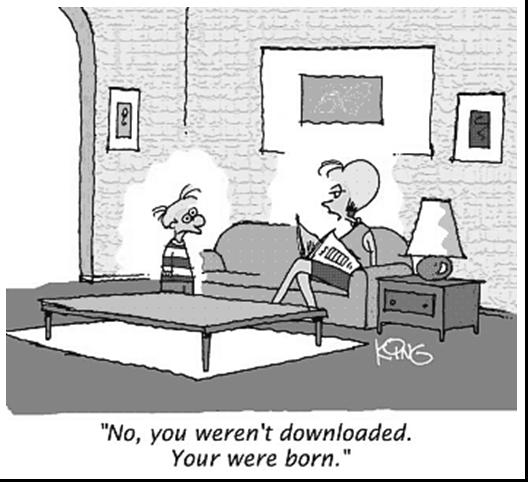
\includegraphics[width=0.85\linewidth]{template_fig1.jpg}
  \caption{[Legenda da figura de resultados]}
  \label{fig:resultados-exemplo}
\end{figure}

% =================================================================
% CAPÍTULO 5: DETALHES DE IMPLEMENTAÇÃO (TEMPLATE)
% Objetivo: registrar decisões técnicas e arquitetura da solução.
% Dicas:
%  - Mantenha diagramas atualizados com o texto.
%  - Use labels descritivos (ex.: fig:diagrama1, lst:prototipo)
% =================================================================
\section{Detalhes de Implementação}

[Descreva detalhes técnicos relevantes da implementação e do design.]

\subsection{Diagrama(s) de Arquitetura}
\begin{figure}[h]
  \centering
  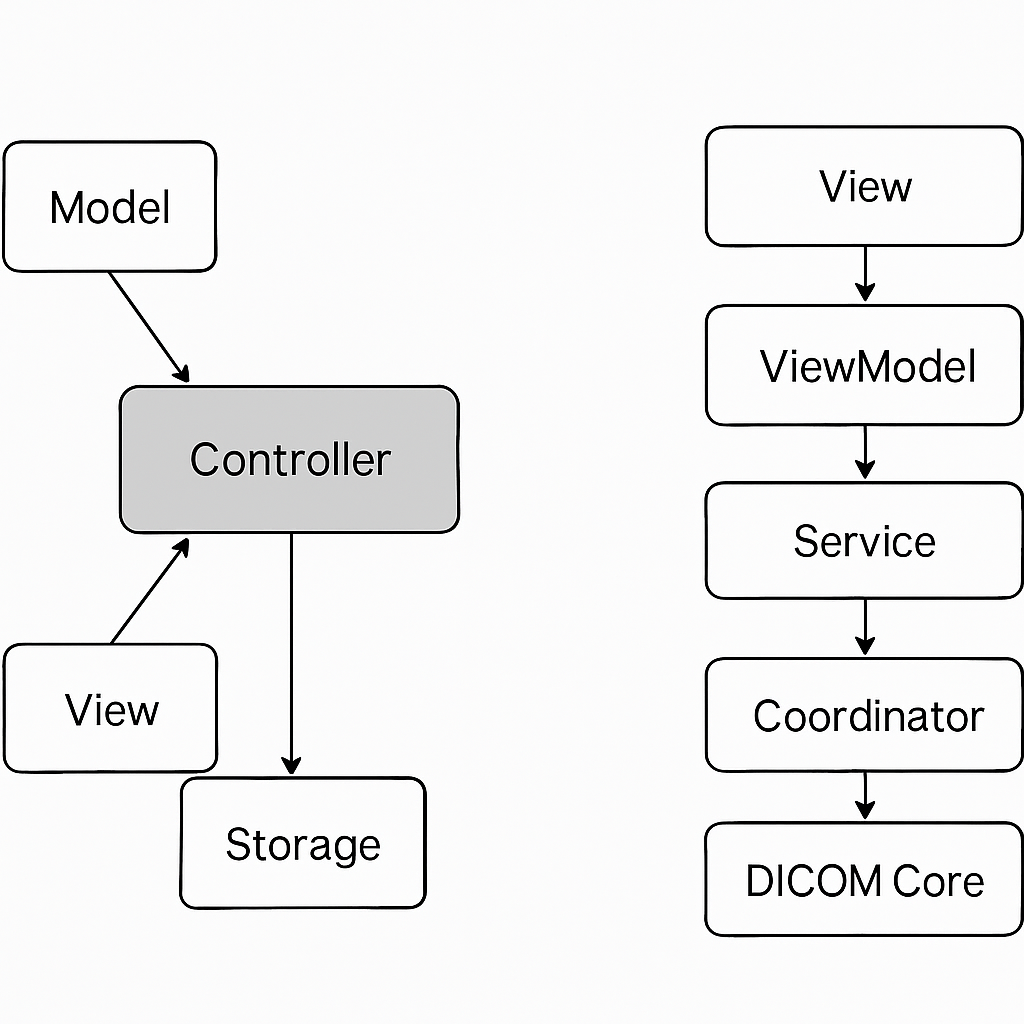
\includegraphics[width=\linewidth]{template_diagram1.png}
  \caption{[Legenda do diagrama 1]}
  \label{fig:diagrama1}
\end{figure}

\begin{figure}[h]
  \centering
  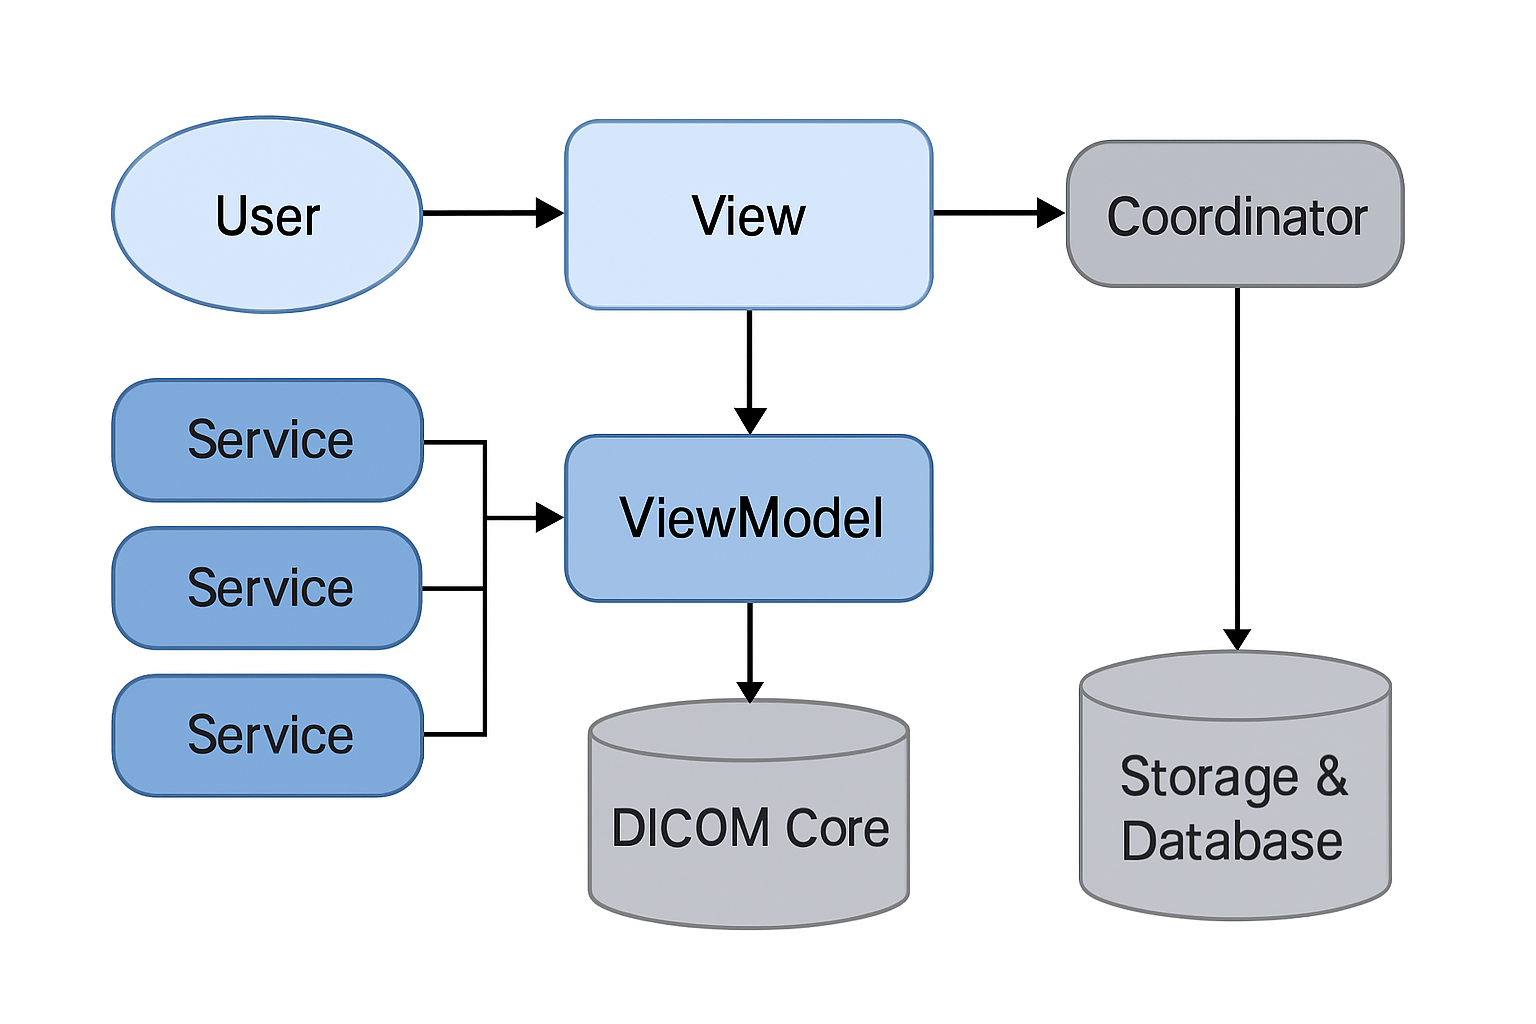
\includegraphics[width=\linewidth]{template_diagram2.png}
  \caption{[Legenda do diagrama 2]}
  \label{fig:diagrama2}
\end{figure}

\subsection{Listagens de Código (Opcional)}
% \begin{lstlisting}[style=code, caption={<Legenda do trecho de código>}, label={lst:<identificador>}]
% <Exemplo de código ou pseudocódigo>
% \end{lstlisting}
[Inclua listagens de código, se aplicável ao trabalho.]

% =================================================================
% CAPÍTULO 6: DESAFIOS TÉCNICOS (TEMPLATE)
% Objetivo: relatar dificuldades, riscos e aprendizados.
% Dicas:
%  - Vincule cada desafio a uma mitigação específica.
%  - Aponte impactos e limitações remanescentes.
% =================================================================
\section{Desafios Técnicos}

[Liste e descreva desafios técnicos relevantes enfrentados durante o trabalho.]

\subsection{Riscos e Mitigações}
[Aponte riscos identificados e estratégias de mitigação.]

\subsection{Lições Aprendidas}
[Registre aprendizados e recomendações.]

% =================================================================
% CAPÍTULO 7: TRABALHOS FUTUROS (TEMPLATE)
% Objetivo: propor continuação, melhorias e pesquisas futuras.
% Dicas:
%  - Diferencie curto/médio/longo prazo.
%  - Relacione com limitações apontadas nas conclusões.
% =================================================================
\section{Trabalhos Futuros}

[Sugira extensões, melhorias e novas linhas de estudo/pesquisa.]

\subsection{Melhorias Incrementais}
[Liste melhorias de curto/médio prazo.]

\subsection{Pesquisas e Extensões}
[Apresente propostas de longo prazo e hipóteses.]

% =================================================================
% CAPÍTULO 8: CONCLUSÕES E CONTRIBUIÇÕES (TEMPLATE)
% Objetivo: fechar argumentos, sintetizar resultados e destacar contribuições.
% Dicas:
%  - Evite introduzir conteúdo novo; foque na síntese.
%  - Separe claramente conclusões, contribuições e limitações.
% =================================================================
\section{Conclusões e Contribuições}

[Resuma as conclusões frente aos objetivos e destaque as contribuições do trabalho.]

\subsection{Conclusões}
[Apresente as principais conclusões e impactos.]

\subsection{Contribuições}
[Detalhe contribuições teóricas, práticas e metodológicas.]

\subsection{Limitações}
[Descreva limitações e ameaças à validade.]


% =================================================================
% AGRADECIMENTOS (OPCIONAL - DESCOMENTE SE NECESSÁRIO)
% =================================================================
% % =================================================================
% ACKNOWLEDGMENTS (OPTIONAL)
% How to use: Include this file at the end of your thesis, before the bibliography.
% In thesis-main.tex, add: % =================================================================
% ACKNOWLEDGMENTS (OPTIONAL)
% How to use: Include this file at the end of your thesis, before the bibliography.
% In thesis-main.tex, add: % =================================================================
% ACKNOWLEDGMENTS (OPTIONAL)
% How to use: Include this file at the end of your thesis, before the bibliography.
% In thesis-main.tex, add: \input{sections/acknowledgments-thesis}
% =================================================================
% Tips: Express gratitude to advisors, funding agencies, colleagues, family, and friends.
% Keep it sincere and professional.

\chapter*{Acknowledgments}
\addcontentsline{toc}{chapter}{Acknowledgments}

[Write your acknowledgments here. Express gratitude to those who contributed directly or indirectly to your research. Include advisors, committee members, funding agencies, research groups, colleagues, family, and friends.]


% =================================================================
% Tips: Express gratitude to advisors, funding agencies, colleagues, family, and friends.
% Keep it sincere and professional.

\chapter*{Acknowledgments}
\addcontentsline{toc}{chapter}{Acknowledgments}

[Write your acknowledgments here. Express gratitude to those who contributed directly or indirectly to your research. Include advisors, committee members, funding agencies, research groups, colleagues, family, and friends.]


% =================================================================
% Tips: Express gratitude to advisors, funding agencies, colleagues, family, and friends.
% Keep it sincere and professional.

\chapter*{Acknowledgments}
\addcontentsline{toc}{chapter}{Acknowledgments}

[Write your acknowledgments here. Express gratitude to those who contributed directly or indirectly to your research. Include advisors, committee members, funding agencies, research groups, colleagues, family, and friends.]



% =================================================================
% SEÇÕES/ANEXOS OPCIONAIS (DESCOMENTE SE PRECISAR)
% =================================================================
% % =================================================================
% APÊNDICES/ANEXOS (OPCIONAL)
% Como usar: inclua este arquivo ao final do documento.
% Em artigos, use \appendix para que as seções sejam rotuladas como A, B, ...
% =================================================================
\appendix

\section{Título do Apêndice}

[Inclua material complementar: questionários, detalhes técnicos extensos, etc.]


% % =================================================================
% CRONOGRAMA (OPCIONAL)
% Como usar: inclua se pertinente ao trabalho (TCC/monografia).
% =================================================================
\section{Cronograma}

% Exemplo de tabela de cronograma (substitua com seu plano)
% \begin{table}[h]
%   \centering
%   \caption{Cronograma de Atividades}
%   \label{tab:cronograma}
%   \begin{tabular}{lcccc}
%     \toprule
%     Atividade & M1 & M2 & M3 & M4 \\
%     \midrule
%     Levantamento bibliográfico & X & X &   &   \\
%     Implementação             &   & X & X &   \\
%     Redação final             &   &   & X & X \\
%     \bottomrule
%   \end{tabular}
% \end{table}

[Descreva marcos, entregas e prazos.]


% % =================================================================
% GUIA RÁPIDO DE LaTeX (EXEMPLOS DIDÁTICOS)
% Como usar: inclua em article-main-v2.tex se desejar.
% =================================================================
\section{Guia Rápido de LaTeX}

\subsection{Citações e Referências}
Use \verb+\cite{chave}+ para citar (ex.: \cite{ref:exemplo}). Use \verb+\label{...}+ e \verb+\ref{...}+ para seções/figuras/tabelas.

\subsection{Figuras lado a lado (subfiguras)}
% Nota: o template SBC usa caption2; evite o pacote caption/subcaption.
% Use minipage e legendas textuais por subfigura, com uma legenda geral.
\begin{figure}[h]
  \centering
  \begin{minipage}{.48\linewidth}
    \centering
    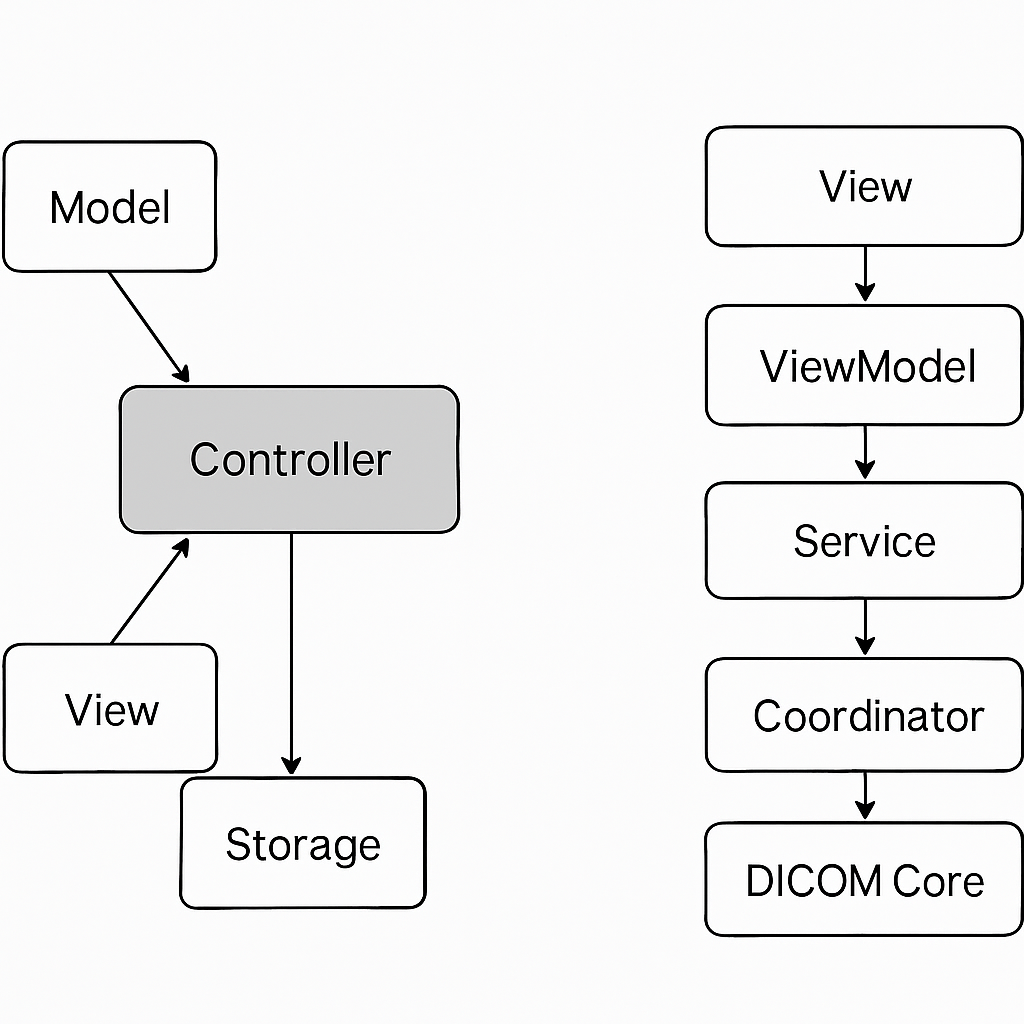
\includegraphics[width=\linewidth]{template_diagram1.png}\\
    \textit{(a) [Subfigura A]}
    \label{fig:sub-a}
  \end{minipage}\hfill
  \begin{minipage}{.48\linewidth}
    \centering
    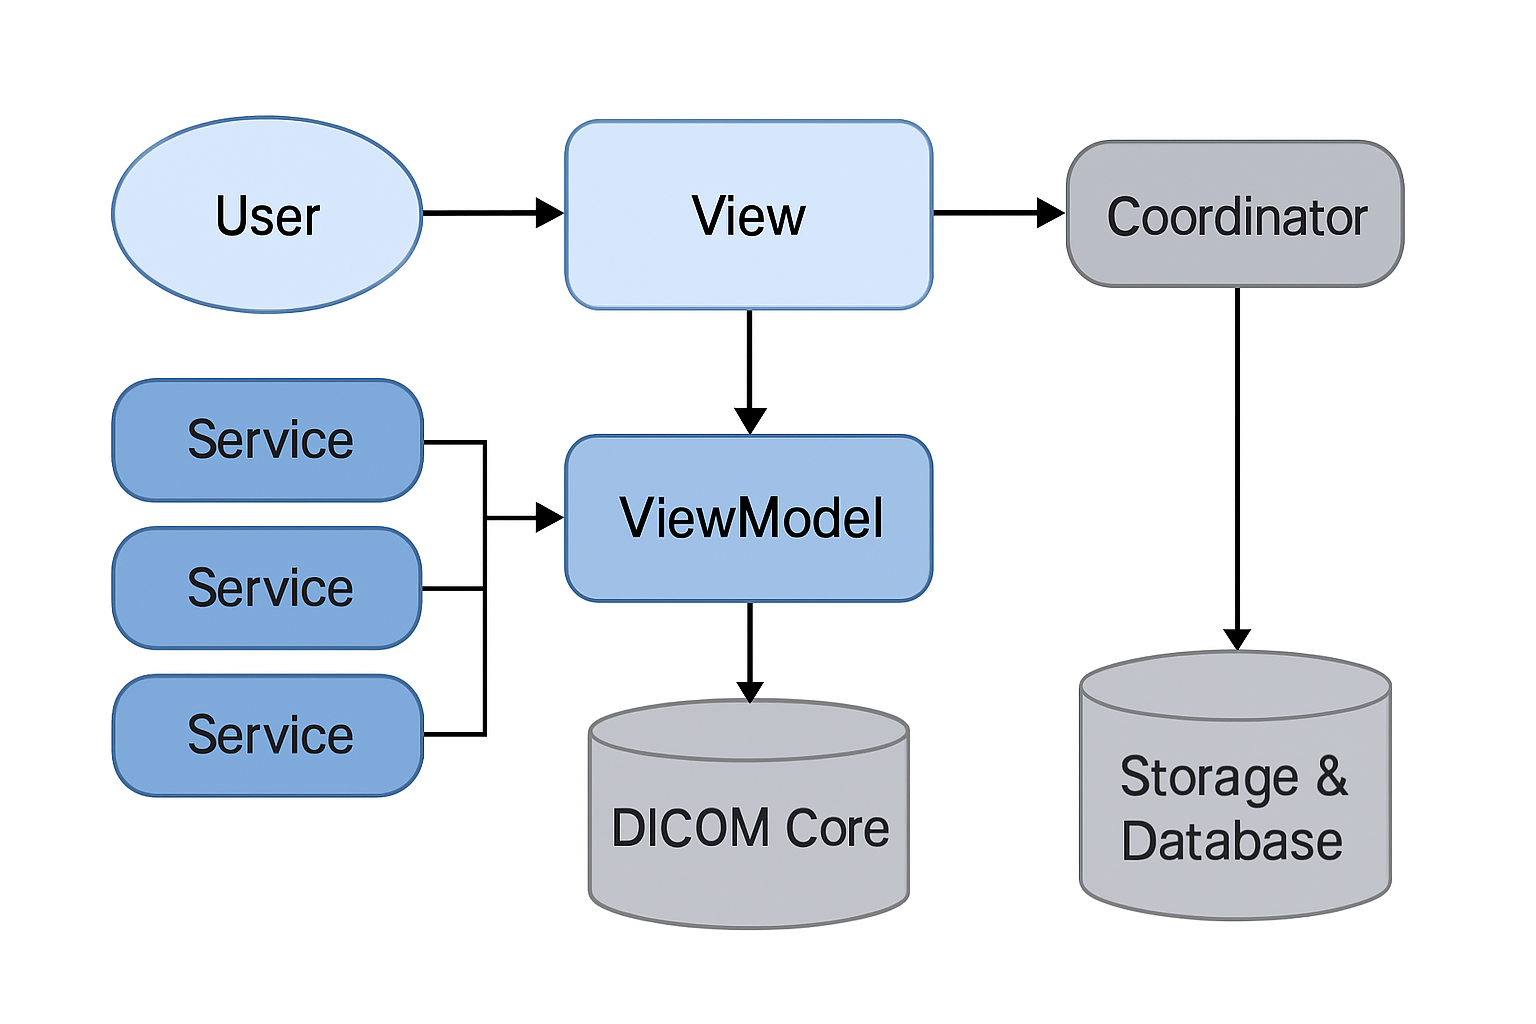
\includegraphics[width=\linewidth]{template_diagram2.png}\\
    \textit{(b) [Subfigura B]}
    \label{fig:sub-b}
  \end{minipage}
  \caption{[Exemplo de figuras lado a lado]}
  \label{fig:subcaption-exemplo}
\end{figure}

\subsection{Tabela Larga com tabularx}
\begin{table}[h]
  \centering
  \caption{[Tabela com colunas flexíveis]}
  \label{tab:tabularx-exemplo}
  \begin{tabularx}{\linewidth}{lXX}
    \toprule
    Campo & Descrição (coluna X) & Observações (coluna X) \\
    \midrule
    A & Texto longo que se ajusta automaticamente à largura disponível & Outra observação longa para demonstração \\
    B & Texto adicional & Mais observações \\
    \bottomrule
  \end{tabularx}
\end{table}

\subsection{Equações Numeradas e Referências}
Uma equação de exemplo em~\eqref{eq:exemplo}:
\begin{equation}
  E = m c^{2}
  \label{eq:exemplo}
\end{equation}

\subsection{Pseudocódigo / Código}
Com \texttt{listings} (não requer shell-escape):
\begin{lstlisting}[style=code, caption={Exemplo com listings}, label={lst:listings-exemplo}]
for i in 1..N {
  // faça algo
}
\end{lstlisting}

% Com minted (opcional) — requer TEXFLAGS="-shell-escape" e \usepackage{minted}
% \begin{minted}[fontsize=\footnotesize, linenos]{python}
% for i in range(10):
%     print(i)
% \end{minted}


% =================================================================
% BIBLIOGRAFIA (ESCOLHA UMA OPÇÃO)
% =================================================================
% Opção A — thebibliography (padrão, simples):
% =================================================================
% BIBLIOGRAFIA
% =================================================================

\begin{thebibliography}{99}

\bibitem{ref:exemplo}
[Autor]. [Título]. [Ano]. [Local/Periódico]. [Editora/DOI/URL].

\end{thebibliography}


% Opção B1 — BibTeX (.bib): comente a linha acima e descomente as duas abaixo.
% Observação: \bibliographystyle{sbc} requer que sbc.bst esteja acessível
% (mova bibliography/sbc.bst para a raiz do projeto se necessário).
% \bibliographystyle{sbc}
% \bibliography{bibliography/sbc-template}

% Opção B2 — biblatex + biber: configure no config/thesis-config.tex
% (descomente o \usepackage[backend=biber]{biblatex} e o \addbibresource{...})
% e então descomente abaixo para imprimir a bibliografia.
% \printbibliography

% Índice remissivo (se habilitado em config/thesis-config.tex)
% \printindex

\end{document}
